\documentclass[a4paper]{book}

% 引用setting里的设置,而不直接写在这里,使代码更简洁
%% packages

\usepackage{blindtext} % needed for creating dummy text passages
%\usepackage{ngerman} % needed for German default language
\usepackage{amsmath} % needed for command eqref
\usepackage{amssymb} % needed for math fonts
\usepackage[
	colorlinks=true
	,breaklinks
	%,ngerman
	]{hyperref} % needed for creating hyperlinks in the document, the option colorlinks=true gets rid of the awful boxes, breaklinks breaks lonkg links (list of figures), and ngerman sets everything for german as default hyperlinks language
%\usepackage[hyphenbreaks]{breakurl} % ben�tigt f�r das Brechen von URLs in Literaturreferenzen, hyphenbreaks auch bei links, die �ber eine Seite gehen (mit hyphenation).
\usepackage{xcolor}
\definecolor{c1}{rgb}{0,0,1} % blue
\definecolor{c2}{rgb}{0,0.3,0.9} % light blue
\definecolor{c3}{rgb}{0.3,0,0.9} % red blue
\hypersetup{
    linkcolor={c1}, % internal links
    citecolor={c2}, % citations
    urlcolor={c3} % external links/urls
}
%\usepackage{cite} % needed for cite
\usepackage[round,authoryear]{natbib} % needed for cite and abbrvnat bibliography style
\usepackage[nottoc]{tocbibind} % needed for displaying bibliography and other in the table of contents
\usepackage{graphicx} % needed for \includegraphics 
\usepackage{longtable} % needed for long tables over pages
\usepackage{bigstrut} % needed for the command \bigstrut
\usepackage{enumerate} % needed for some options in enumerate
\usepackage{todonotes} % needed for todos
\usepackage{makeidx} % needed for creating an index
\usepackage[UTF8, heading=true]{ctex}
\makeindex
  
%% page settings

\usepackage[top=2cm, bottom=1.8cm,left=2.5cm,right=2.5cm]{geometry} % needed for page border settings
\parindent=2cm % for space of first line of new text block
\sloppy % for writing with hyphenless justification (tries to)
\hyphenation{} % 让连接词不出现在同一行
\hyphenpenalty=10000
\exhyphenpenalty=10000
\usepackage{fancyhdr} % 页眉页脚设定

%% my macros

%% Text fomats
\newcommand{\tbi}[1]{\textbf{\textit{#1}}}

%% Math fonts
\newcommand{\bbA}{\mathbb{A}}
\newcommand{\bbB}{\mathbb{B}}
\newcommand{\bbC}{\mathbb{C}}
\newcommand{\bbD}{\mathbb{D}}
\newcommand{\bbE}{\mathbb{E}}
\newcommand{\bbF}{\mathbb{F}}
\newcommand{\bbG}{\mathbb{G}}
\newcommand{\bbH}{\mathbb{H}}
\newcommand{\bbI}{\mathbb{I}}
\newcommand{\bbJ}{\mathbb{J}}
\newcommand{\bbK}{\mathbb{K}}
\newcommand{\bbL}{\mathbb{L}}
\newcommand{\bbM}{\mathbb{M}}
\newcommand{\bbN}{\mathbb{N}}
\newcommand{\bbO}{\mathbb{O}}
\newcommand{\bbP}{\mathbb{P}}
\newcommand{\bbQ}{\mathbb{Q}}
\newcommand{\bbR}{\mathbb{R}}
\newcommand{\bbS}{\mathbb{S}}
\newcommand{\bbT}{\mathbb{T}}
\newcommand{\bbU}{\mathbb{U}}
\newcommand{\bbV}{\mathbb{V}}
\newcommand{\bbW}{\mathbb{W}}
\newcommand{\bbX}{\mathbb{X}}
\newcommand{\bbY}{\mathbb{Y}}
\newcommand{\bbZ}{\mathbb{Z}}

%%%%%%%%%%%%%%%%%%%%%%%%%%%%%%%%%%%%%%%%%%%
\usepackage{hyperref}%设置超链接
\hypersetup{colorlinks, linkcolor=blue}
\usepackage{graphicx}
\usepackage{color}
\usepackage{mboxfill}
\usepackage{ctex}
\usepackage{amsmath}
\usepackage{lipsum} %随机文本
\usepackage{pifont}
\usepackage{amsthm}
\usepackage{caption}
%%%%%%%%%%%%%%%%%%%%%%%%%%%%%%%%%%%%%%%%%%%
\newcommand{\xtjc}[1]{\textbf{\textit{#1}}}
\renewcommand{\proofname}{\indent\bf 证明}%将证明两个字加粗
\makeatletter
\renewenvironment{proof}[1][\proofname]{\par
	\pushQED{\qed}%
	\normalfont \topsep6\p@\@plus6\p@\relax
	\trivlist
	\item[\hskip\labelsep
	\itshape
	#1\@addpunct{}]\ignorespaces
}{%
	\popQED\endtrivlist\@endpefalse
}
\makeatother   %去掉证明环境中证明两字后面的.
\captionsetup[figure]{labelsep=space}
%%%%%%%%%%%%%%%%%%导言区%%%%%%%%%%%%%%%%%%%


\begin{document}

% downloaded template
\begin{titlepage}

\newcommand{\HRule}{\rule{\linewidth}{0.5mm}} % 定义横线
\center % Center everything on the page
 
%----------------------------------------------------------------------------------------
%	HEADING SECTIONS
%----------------------------------------------------------------------------------------

\textsc{\LARGE Wuhan University}\\[1.5cm] % Name of your university/college


%----------------------------------------------------------------------------------------
%	TITLE SECTION
%----------------------------------------------------------------------------------------

\HRule \\[0.4cm]
{ \LARGE \bfseries Duality of the Two-Dimensional Ising Model }\\[0.4cm] % Title of your document
\HRule \\[1.5cm]
 
%----------------------------------------------------------------------------------------
%	AUTHOR SECTION
%----------------------------------------------------------------------------------------

\begin{minipage}{0.4\textwidth}
 \centering{\Large\textbf{猫の薛定谔} }
\end{minipage}


\vfill % Fill the rest of the page with whitespace
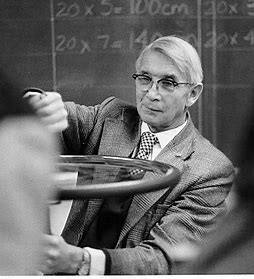
\includegraphics[width=0.6\textwidth]{figures/伊辛}\\[1cm]
\end{titlepage}



\pagestyle{plain}
\centerline{\LARGE{\textbf{前言}}}\par 
~\par
在前面讨论班的学习中,我们引入了平均场近似的方法来求解一维Ising模型,而本章我们将正式进入二维Ising模型的求解.在二维模型中有一个相变,其临界指数与在平均场近似中得到的值不同.因此,它提供了临界现象的一个重要例子.我们将非常详细地看到,在所有精确求解的统计力学模型中,二维伊辛模型不仅是研究最多的,而且也是证明了一系列深刻的数学和物理结果的模型。该模型的许多解因其使用的巧妙方法而脱颖而出,如行列式理论、组合方法、Grassmann变量或椭圆函数.许多结果深刻地影响了对关键现象的理解,并强烈地激发了新的研究领域。在研究二维伊辛模型中成熟的思想,例如其高温相和低温相之间的对偶性,已经被推广到其他力学统计系统中,并且也在其他重要领域中找到了重要和基本的应用,例如量子场论.同样重要的发现是,在临界点附近,模型的动力学可以用所谓的马约拉纳费米子的相对论性Dirac方程来描述.\par 
本次讨论课致力于研究一些可以通过基本方法与假设来建立的模型的性质.我们特别讨论了Peierls证明模型中存在相变的论点。我们还给出了方形晶格的低温配分函数和高温配分函数、三角晶格配分函数和六角晶格的配分函数之间的对偶关系.在最后一种情况下我们引入了一个恒等式,即\xtjc{star–triangle equation},它将在以后的研究中大放异彩.\par 
最后感谢各位同学参加讨论班,由于本人水平有限,写的东西与其说是讲义,不如说是我个人的学习笔记.缺点和疏漏在所难免,恳请大家不吝指正,万分感激!
\newpage
%%%%%%%%%%%%%%%%%%%%%%%%%%%%%%%%%%%%%%%%%%%%%%%%%%%%%%%%%%%
\tableofcontents%封面


%%%%%%%%%%%%%%%%%%%%%%%%%%%%%%%%%%%%%%%%%%%%%%%%%%%%%%%%%%%
%%%%%%%%%%%%%%%%%%%%%%%%%%%%%%%%%%%%%%%%%%%%%%%%%%%%%%%%%%%
%%%%%%%%%%%%%%%%%%%%%%%%%%%%%%%%%%%%%%%%%%%%%%%%%%%%%%%%%%%


\chapter{Peierls 的观点}
1936年,Peierls证明了二维或高维的伊辛模型有一个低温区,其中自发磁化不等于零.由于系统在高温下是无序的,因此必然存在一个发生相变的临界温度$T_c$.\par 
Peierls认为每个相变都对应到一组的闭合区域(图1.1),这些虚线将自旋为$-1$的区域与自旋为$+1$的区域分开来.如果我们能够证明在足够低的温度下,封闭线包围的区域大小的平均值仅占系统总体积的一小部分,我们就可以证明大多数自旋普遍处于自发磁化的状态.
 \begin{figure}[!h]
	\centering
	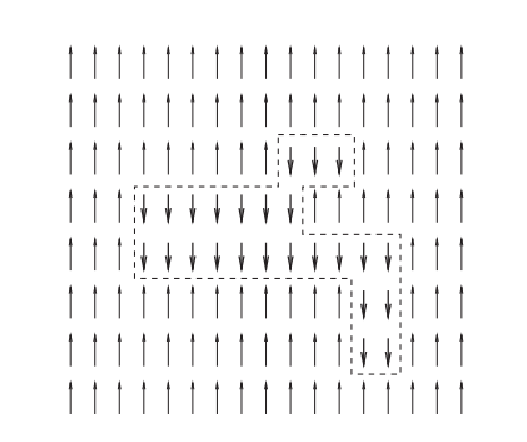
\includegraphics[width=7cm,height=5.5cm]{figures/1.eps}
	\caption{虚线框住的区域表示自旋翻转的区域.}
\end{figure}
现考虑低温下的Ising模型,假设处于最低能量下的粒子自旋都为$+1$,则温度涨落将会导致部分粒子自旋发生变化,引起这部分变化的能量损耗为
\begin{equation}\label{1.1}
	\varDelta E=2JL
\end{equation}
其中$L$为虚线区域长度.\par 
那么现在的问题是对于一个给定的$L$.这个框的位置可以在晶体的任意区域,并且框的形状也是任意的.故为了简化,我们认为这个框是在给定区域中随机走$L$步得到的,并且每步仅有两种结果,尽管二维方形模型下每步有四种结果,并且其得到的熵值也是最大的,但这种走法忽略了虚线区域的闭合性.故在走完$L$步后系统总的状态数$\Omega$为$2^L$,故涨落带来熵的变化为
\begin{equation}
	\varDelta S=k\,ln2^L=kL\,ln2
\end{equation}
故自由能的变化为
\begin{equation}
	\varDelta F=\varDelta E-T\varDelta S=L(2J-kT\,ln2)\geq0
\end{equation}
故系统当中发生该情况的变化的条件为
\begin{equation}\label{1.4}
	T\leq T_c=\frac{2J}{k\,ln2}\approx2.885\frac{J}{k}
\end{equation}
这个值与实际临界温度值十分接近!
\let\cleardoublepage\clearpage %去掉空白页
\chapter{方形晶体中的对偶关系}
Peierls的论证表明二维Ising模型有两个不同的情况:无序的高温情况和有序的低温情况.Kramers和Wannier首先利用高温配分函数和低温配分函数之间的对偶关系确定了发生相变的临界温度.而二维方形晶体中的对偶性是其最为重要的性质之一.在引入对偶关系之前,我们先学习模型在高温和低温下的级数展开.
\section{高温展开}
现考虑一个方形格子$\mathcal{L}$,其有$M$个水平连接和$M$个竖直连接.在$M\rightarrow\infty$时$M$就等于晶体的格点数$N$.现在我们要试着写出其Hamiltonian,由于水平和竖直方向的耦合常数不同,我们分别用$J$和$J'$代表水平和竖直方向的耦合常数.此时配分函数为
\begin{equation}\label{2.1}
	Z_N=\sum_{\{\sigma\}}exp\Big[K\sum_{(i,j)}\sigma_i\sigma_j+L\sum_{(i,k)}\sigma_i\sigma_k\Big]
\end{equation}
其中
\begin{equation}
	K=\beta J
\end{equation}
\begin{equation}
	L=\beta J'
\end{equation}
由于
\begin{equation}
	exp[x\sigma_i\sigma_j]=\frac{e^x+e^{-x}}{2}+\frac{e^x-e^{-x}}{2}\sigma_i\sigma_j=coshx(1+\sigma_i\sigma_jtanhx)
\end{equation}
故配分函数可以写为
\begin{equation}\label{2.5}
	Z_N=(coshKcoshL)^M\sum_{\{\sigma\}}\prod_{(i,j)}(1+v\sigma_i\sigma_j)\prod_{(i,k)}(1+w\sigma_i\sigma_k)
\end{equation}
其中$v=tanhK,w=tanhL$.在高温情况下,各个格点的自旋情况是独立的,也就意味着我们直接进行求和是行不通的.但不难发现,由于$K,L\ll1$,故可以得到$v,w\ll1$.所以在$T\rightarrow\infty$时我们可以将$v$和$w$进行级数展开,故称其为\textbf{高温展开}.\par 
现考虑每一个$(1+v\sigma_i\sigma_j)$和$(1+w\sigma_i\sigma_k)$,其分别代表了一对水平连接$(i,j)$和竖直连接$(i,k)$,若两点之间没有连接,则上面两项的取值都为1,换句话说,\hyperref[2.5]{2.5}式当中做乘积的每一项都代表了一组相邻格点之间的连接(尽管它们两个之间可能并没有发生连接).而\hyperref[2.5]{2.5}式中我们将乘积展开共有$2^{2M}$项,因为总共有$2M$个连接,而每个连接会带来两项(分别是1和含$\sigma$项).那么每一项的形式就为
\begin{equation}\label{2.6}
	v^rw^s\sigma_1^{n_1}\sigma_2^{n_2}\sigma_3^{n_3}...\sigma_N^{n_N}
\end{equation}
其中$r$为水平的连接数,$s$为竖直的连接数,$n_i$代表第$i$个结点上连接的数目.由于$\sigma_i=\pm1$,若$n_i$为奇数,则在后续的求和中奇数项就会被抵消掉,故只有所有的$n_i$都取偶数时该项才会被保留下来,若转为图式法的语言,也就意味着只有偶数次连接的格点才会对配分函数做出贡献,换句话说,这个连线必须是\textbf{闭合}的!\par 
通过以上讨论,我们就可以得到
\begin{equation}\label{2.7}
	Z_N=2^N[coshKcoshL]^M\sum_{p}v^rw^s
\end{equation}
其中$2^N$是由于对于指定$r$和$s$的一组\hyperref[2.6]{2.6}式,其中共有$2^N$种可能的$\sigma$的组合.现在$\sum$代表对$\mathcal{L}$中有偶数次连线的格点求和.故现在我们只需要考虑
\begin{equation}
	\varPhi=\sum_{p}v^rw^s
\end{equation}
对于$\varPhi$的第一项,$\varPhi=1$,代表的是各个格点之间没有连接;第二项为$(vw)^2$,其构成的为一个面积为1的方格,即$1\times$1大小的方格,而我们可以在任意一个格点上绘制这个方格,故总共有N个方格,总的求和就为$N(vw)^2$;而第三项自然对应的为面积为2的方格,有两种,即1$\times$2或2$\times$1,分别有N个,故总贡献为$N(v^2w^4+v^4w^2)$.以此类推,$\varPhi$可以写为
\begin{equation}
	\varPhi=1+N(vw)^2+N(v^2w^4+v^4w^2)+...
\end{equation}
尽管我们可以不断的写下去,但实际上我们没有必要这么做,因为我们所需要的对偶性质已经可以通过\hyperref[2.7]{2.7}式得到了.
\section{低温展开}
在低温的情况下,根据Peierls的观点,自旋总是趋向于相互平行的方向排列的.但总有一些格点的自旋是和相邻的格点是反平行的.我们不妨假设低温下大多数格点自旋向上,令$r$为自旋反平行的竖直连接,$s$为自旋反平行之间的水平连接.则相邻自旋平行的竖直连接和水平连接分别有$M-r$个和$M-s$个.此时\hyperref[2.1]{2.1}式可写为
\begin{equation}\label{2.10}
	Z_N=\sum_{\{\sigma\}}exp[K(M-2s)+L(M-2r)]
\end{equation}
故配分函数仅依赖于$r$和$s$,为了进一步简化,我们需引入\textbf{对偶晶格}的概念.对于晶格$\mathcal{L}$,定义其对偶晶格$\mathcal{L}_D$,其格点位于原始晶格各个格子的中心.对于方形格子,其对偶晶格仍为方形格子(图2.1).
 \begin{figure}[!h]
	\centering
	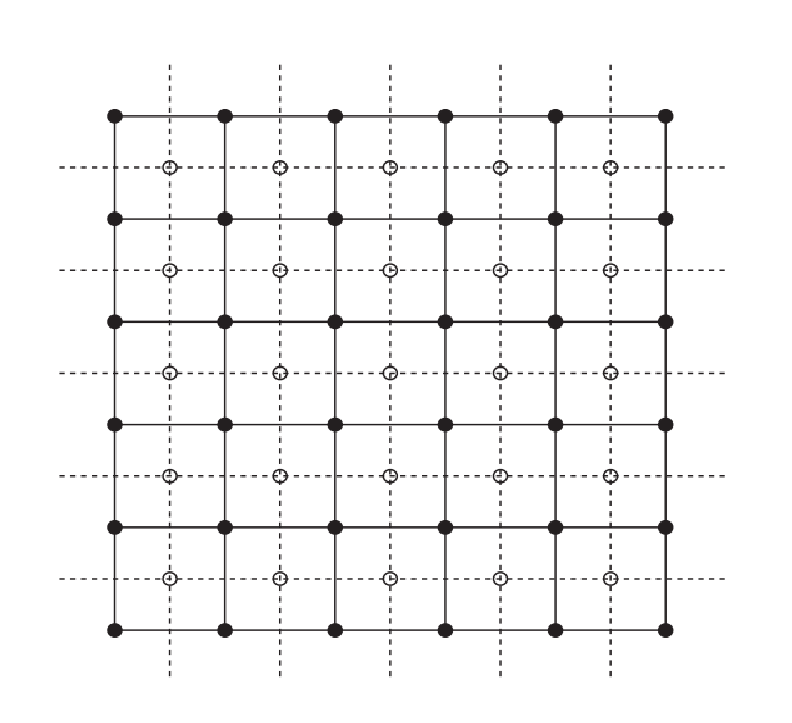
\includegraphics[width=7cm,height=6.5cm]{figures/2.eps}
	\caption{方形晶格的对偶晶格.}
\end{figure}
借助对偶晶格,我们就可以用类似高温展开的方法去连线.若原始晶格中相邻两个格点自旋平行,则两个格点连线两侧的对偶晶格的格点就不连线,反之就连线(图2.2).
 \begin{figure}[!h]
	\centering
	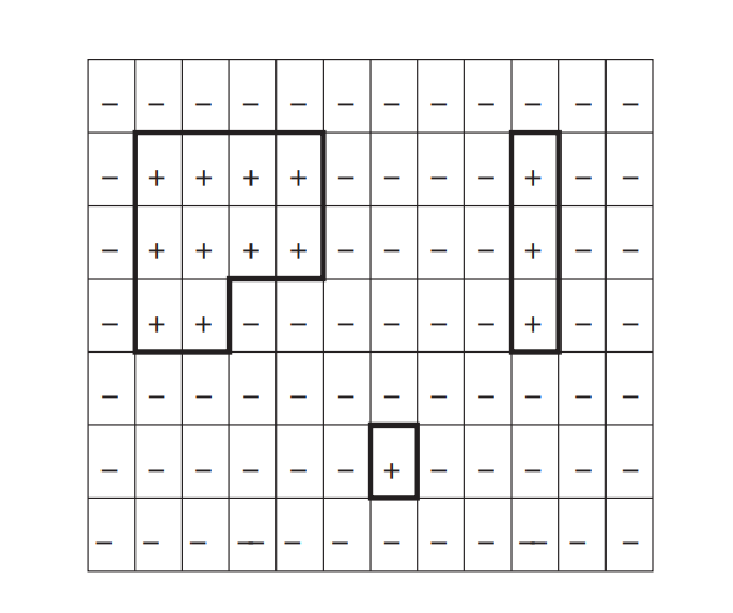
\includegraphics[width=7cm,height=6.5cm]{figures/3.eps}
	\caption{}
\end{figure}
现在我们来看看$r$和$s$的含义,每出现一对反平行的格点,对偶晶格中就需要连接一对格点,不难发现$r$代表的是对偶晶格中水平方向的连接,$s$代表的是竖直方向的连接.故\hyperref[2.10]{2.10}式可写为
\begin{equation}
	Z_N=exp[M(K+L)]\sum_{\tilde{p}}exp[-2Lr-2Ks]
\end{equation}
类似地,$\tilde{p}$代表的是对偶晶格中被连接偶数次的格点.故我们也仅需考虑函数
\begin{equation}
	\tilde{\varPhi}(e^{-2L},e^{-2K})=\sum_{\tilde{p}}exp[-2Lr-2Ks]
\end{equation}
自然地,其可以展开为
\begin{equation}
\tilde{\varPhi}(e^{-2L},e^{-2K})=1+Ne^{-4L-4K}+N(e^{-4L-8K}+e^{-8L-4K})+...
\end{equation}
我们将这种展开称为低温展开.
\section{自对偶性}
为了构建我们想要的关系式,我们不妨从原始晶格出发,在这个晶格上画一个具有r个连接的闭合图形.我们构建它的对偶晶格,并且在图形内部进行自旋翻转,我们会发现相邻格点自旋相反的连接为r个时的可能数与原始晶格上r个连接的可能数是相同的!反之亦然.这表面给定晶格的某种图形与对偶晶格的另一种图形有一一对应的关系.换句话说,若我们指定原始晶格中$(r,s)$的取值,对偶晶格中自旋相反晶格的连接情况也为$(r,s)$.\par 
若考虑原始晶格在高温$T$情况下,其配分函数为
\begin{equation}
		Z_N^{H}=2^N[coshKcoshL]^M\sum_{p}v^rw^s
\end{equation}
并且考虑其对偶晶格处于低温$\tilde{T}$下,配分函数为
\begin{equation}
		\tilde{Z_N^{L}}=exp[M(\tilde{K}+\tilde{L})]\sum_{\tilde{p}}exp[-2\tilde{L}r-2\tilde{K}s]
\end{equation}
若$M\rightarrow\infty$,则$N=M$.我们对两者分别求平均自由能可知
\begin{equation}
	\frac{lnZ}{N}=ln2+ln(coshKcoshL)+g(v,w)=M(\tilde{K}+\tilde{L})+g(e^{-2\tilde{L}},e^{-2\tilde{K}})
\end{equation}
其中$g$代表该级数的对数.g包括了自由能的奇异部分,那么我们很自然的可以想到这样的对应关系
\begin{equation}
	v=e^{-2\tilde{L}},w=e^{-2\tilde{K}}
\end{equation}
即
\begin{equation}\label{2.18}
	sinh2Ksinh2\tilde{L}=1,sin2\tilde{K}sinh2L=1
\end{equation}
上述关系式被称为\textbf{对偶条件}.若我们考虑的是均匀的晶格,即$K=L,\tilde{K}=\tilde{L}$,若$g(k)$在$K=K_c$下具有奇异性(配分函数发散),则其必然也在$\tilde{K}=K_c$下具有奇异性,因为自由能的奇异点仅有一个\footnote[1]{\href{https://journals.aps.org/pr/abstract/10.1103/PhysRev.87.404}{C. N. Yang and T. D. Lee (1952). Phys. Rev. 87, 404. }},即具有自发对偶的性质(可以联想到方格的对偶晶格也是方格),故
\begin{equation}
	tanhK_c=e^{-2K_c}
\end{equation}
解得$T_c\approx2.27J$.
 \begin{figure}[!h]
	\centering
	\includegraphics[width=6.5cm,height=5.5cm]{figures/4.eps}
	\caption{}
\end{figure}
根据\hyperref[2.18]{2.18},我们可以得到
\begin{equation}
		sinh2Ksinh2L=\frac{1}{sin2\tilde{K}sinh2\tilde{L}}
\end{equation}
这意味着高温$T$下的原始晶格与其处于低温$\tilde{T}$下的对偶晶格形成了一种对偶关系.并且我们可以得到它们两者之间配分函数的关系
\begin{equation}
Z^{H}_N=2^N[sinhKsinhL]^M\tilde{Z^L_N}	
\end{equation}
这也被称为\textbf{对偶变换}.
\chapter{六角晶体和三角晶体的对偶关系}
方格晶体中的对偶变换可以推广至其他类型的晶体中.最为典型的就是三角晶体和六角晶体的对偶,它们互为对偶晶格(图3.1).本章就讨论在三角形和六边形晶格上定义的Ising模型的低温和高温之间的映射
 \begin{figure}[!h]
	\centering
	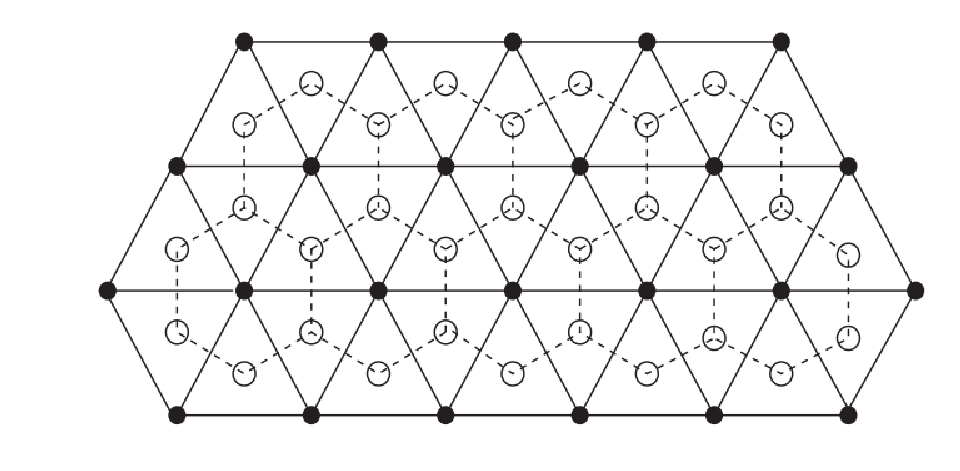
\includegraphics[width=9.5cm,height=4.5cm]{figures/5.eps}
	\caption{六角晶格和三角晶格互为对偶晶格.}
\end{figure}
我们分别令$K_i$和$L_i$($i=1,2,3$)分别为三角和六角晶格的耦合常数.在无外磁场时,六角晶格的配分函数为
\begin{equation}
	Z_N^H(\mathcal{L})=\sum_{\{\sigma\}}exp[\mathcal{L}_1\sum \sigma_l\sigma_i+\mathcal{L}_2\sum \sigma_l\sigma_j+\mathcal{L}_3\sum \sigma_l\sigma_k]
\end{equation}
其中$\mathcal{L}_i=L_i/kT$.指数项内的求和为三条不同方向边的相邻相互作用的格点进行求和.类似地,我们也可以写出三角晶格在无外磁场下的配分函数
\begin{equation}
	Z_N^T(\mathcal{K})=\sum_{\{\sigma\}}exp[\mathcal{K}_1\sum \sigma_l\sigma_i+\mathcal{K}_2\sum \sigma_l\sigma_j+\mathcal{K}_3\sum \sigma_l\sigma_k]
\end{equation}
其中$\mathcal{K}_i=K_i/kT$.我们先考虑三角晶格的高温展开:
\begin{equation}
	Z_N^T(\mathcal{K})=(2cosh\mathcal{K}_1cosh\mathcal{K}_2cosh\mathcal{K}_3)^N\sum_{p}v^{r_1}_1v^{r_2}_2v^{r_3}_3
\end{equation}
其中$v_i=tanh\mathcal{K}_i$,求和代表的为对三角晶格中封闭的格点求和,且沿三个不同方向的边求和.同样的,对六角晶格进行低温展开,对于N个格点的三角晶格其每个格点平均占有的六角晶格的格点为2个,故三角晶格对偶的六角晶格中总共有2N个格点,故
\begin{equation}
	Z_{2N}^H(\mathcal{L})=e^{[N(\mathcal{L}_1+\mathcal{L}_2+\mathcal{L}_3)]}\sum_{p}exp^{[-2(\mathcal{L}_1r_1+\mathcal{L}_2r_2+\mathcal{L}_3r_3)]}
\end{equation}
若三角晶格处于温度$T^*$时,它们具有类似的对偶条件
\begin{equation}\label{3.5}
	tanh\mathcal{K}_i^*=exp[-2\mathcal{L}_i],~i=1,2,3
\end{equation}
由此可以得到
\begin{equation}\label{3.6}
	sinh2\mathcal{K}_i^*sinh2\mathcal{L}_i=1
\end{equation}
且三角晶格的配分函数与六角晶格的配分函数的变换关系为
\begin{equation}\label{3.7}
	Z^{H}_{2N}(\mathcal{L})=(2a_1a_2a_3)^{\frac{N}{2}}Z^{T}_N(\mathcal{K}^*)
\end{equation}
其中$a_i=sinh2\mathcal{L}_i=1/sinh2\mathcal{K}^*_i,i=1,2,3$.\par 
与方形晶格一样,上式表明,当其中一个耦合常数较小时,另一个耦合常数较大,反之亦然。然而,在这种情况下,对偶关系本身不能确定两个晶格的临界温度,因为它们不是自对偶的.幸运的是,在两个晶格的耦合常数之间还存在一个重要的恒等式,即,\xtjc{star-triangle~identity}.这使我们能够确定两个模型的自由能奇点.值得一提的是,star-triangle~identity最初是在电线网络发展而来的,它表示在一个网络中一个星形或一个三角形上排列的三个电阻之间的等价性.
\chapter{Star-Triangle Identity}
六角晶格的配分函数可写为
	\begin{equation}
		Z_N^H(\mathcal{L})=\sum_{\{\sigma\}}exp[\mathcal{L}_1\sum \sigma_l\sigma_i+\mathcal{L}_2\sum \sigma_l\sigma_j+\mathcal{L}_3\sum \sigma_l\sigma_k]
	\end{equation}
	 \begin{figure}[!h]
		\centering
		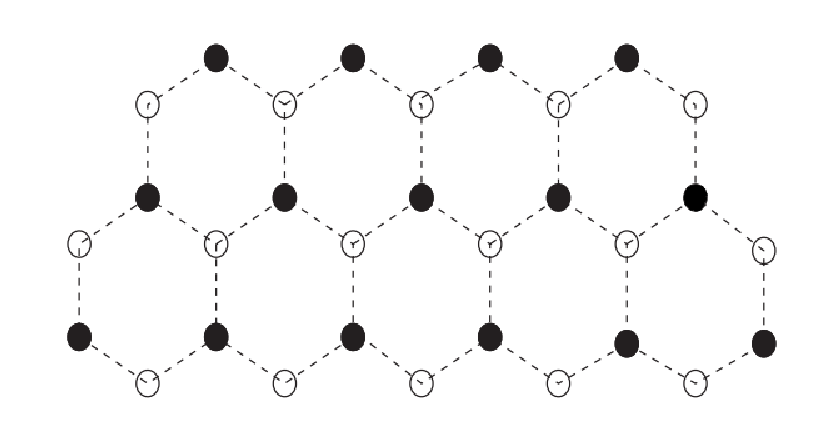
\includegraphics[width=9.5cm,height=4.5cm]{figures/6.eps}
		\caption{图中黑色的为A类点,白色的为B类点.}
	\end{figure}
若我们将六角晶格的格点分为A、B两类(图4.1),且考虑到
\begin{equation}
	\sum_{\{\sigma\}}=\sum_{\sigma_1=\pm1}\sum_{\sigma_2=\pm1}\sum_{\sigma_3=\pm1}...\sum_{\sigma_N=\pm1}=\sum_{\{\sigma_a\}}\sum_{\{\sigma_b\}}
\end{equation}
若取配分函数中的$\sigma_l$为B类中的格点,则相邻求和的格点均为A类的格点.故配分函数亦可写为
\begin{equation}\label{4.3}
		Z_N^H(\mathcal{L})=\sum_{\{\sigma_a\}}\sum_{\sigma_l}\prod_{i,j,k}exp[\sigma_l(\mathcal{L}_i\sigma_i+\mathcal{L}_2\sigma_j+\mathcal{L}_3\sigma_k)]=\sum_{\{\sigma_a\}}\prod_{i,j,k}w(\sigma_i,\sigma_j,\sigma_k)
\end{equation}
其中
\begin{equation}
	w(\sigma_i,\sigma_j,\sigma_k)=\sum_{\sigma_l}exp[\sigma_l(\mathcal{L}_1\sigma_i+\mathcal{L}_2\sigma_j+\mathcal{L}_3\sigma_k)]
\end{equation}
又由于$\sigma_l$的取值仅有1或$-1$,故
\begin{equation}
	w=2cosh[\mathcal{L}_1\sigma_i+\mathcal{L}_2\sigma_j+\mathcal{L}_3\sigma_k]
\end{equation}
又考虑到$w$可以写成含Boltzmann因子的形式,即存在参数$\mathcal{K}_i$和常数$\mathcal{R}$,使得
\begin{equation}\label{4.6}
	w=\mathcal{R}\,exp[\mathcal{K}_1\sigma_j\sigma_k+\mathcal{K}_2\sigma_i\sigma_k+\mathcal{K}_3\sigma_i\sigma_j]
\end{equation}
将\hyperref[4.6]{4.6}式代入\hyperref[4.3]{4.3}式中,且考虑到对$(i,j,k)$求积仅有$N/2$个,可得
\begin{equation}
		Z_N^H(\mathcal{L})=R^{N/2}\sum_{\{\sigma_a\}}\prod_{i,j,k}exp[\mathcal{K}_1\sigma_j\sigma_k+\mathcal{K}_2\sigma_i\sigma_k+\mathcal{K}_3\sigma_i\sigma_j]
\end{equation}
注意到右边不正是三角晶格配分函数的形式嘛,并且考虑到此时$(i,j,k)$都为三角晶体的格点,并且重新选取格点数$N\rightarrow2N$故可得
\begin{equation}\label{4.8}
		Z_{2N}^H(\mathcal{L})=R^NZ^T_N(\mathcal{K})
\end{equation}
这个式子就是著名的star-triangle identity.现在我们要做的就是确定$\mathcal{R}$的取值,经过漫长的计算\footnote{Baxter,R.J (1982). Exactly Solved Models in Statistical Mechanics.},我们可以到
\begin{equation}
	sinh2\mathcal{K}_isinh\mathcal{L}_i=h^{-1}~,i=1,2,3
\end{equation}
\begin{equation}
	\mathcal{R}^2=2h\,sinh\mathcal{L}_1sinh\mathcal{L}_2sinh\mathcal{L}_3
\end{equation}
\begin{equation}\label{4.11}
	h=\frac{(1-v^2_1)(1-v^2_2)(1-V^2_3)}{4[(1+v_1v_2v_3)(v_1+v_2v_3)(v_2+v_3v_1)(v_3+v_1v_2)]^{\frac{1}{2}}}
\end{equation}
其中$v_i=tanh\mathcal{K}_i$.在下一章我们会看到,这些结论的重要意义就是将三角晶格高温和低温的配分函数联系起来.
\chapter{三角晶格与六角晶格的临界温度}
若考虑处于低温下的六角晶格,根据\hyperref[3.7]{3.7}式,有
\begin{equation}
	Z^{H}_{2N}(\mathcal{L})=(2a_1a_2a_3)^{\frac{N}{2}}Z^{T}_N(\mathcal{K}^*)
\end{equation}
其中$a_i=sinh2\mathcal{L}_i$.而$Z^{T}_N(\mathcal{K}^*)$代表高温下三角晶格的配分函数.
又根据\hyperref[4.8]{4.8}式可得
\begin{equation}
	Z_{2N}^H(\mathcal{L})=R^NZ^T_N(\mathcal{K})
\end{equation}
此处$Z^{T}_N(\mathcal{K})$为低温下三角晶格的配分函数.那么我们立马就可以建立起两者的关系
\begin{equation}
	Z^T_N(\mathcal{K})=h^{-N/2}Z^{T}_N(\mathcal{K}^*)
\end{equation}
且
\begin{equation}\label{5.4}
	sinh2\mathcal{K}^*=h\,sinh\mathcal{K}
\end{equation}
若我们考虑的三角晶体是均匀的,即$\mathcal{K}_1=\mathcal{K}_2=\mathcal{K}_3=\mathcal{K}$,则当处于临界温度时,根据\hyperref[5.4]{5.4}式,$h=1$,故\hyperref[4.11]{4.11}式可写为
\begin{equation}
		1=\frac{(1-v^2)^3}{4[(1+v^3)v^3(1+v)^3]^{\frac{1}{2}}}
\end{equation}
解得$v_c=2-\sqrt{3}$.即$tanh\frac{\mathcal{K}}{kT_c}=2-\sqrt{3}$,由此可得
\begin{equation}
	T^{tr}_c\approx3.64\mathcal{K}
\end{equation}
又根据\hyperref[3.6]{3.6}式我们可以得到六角晶格的临界温度
\begin{equation}
	sinh\frac{2\mathcal{L}}{kT_c}=\sqrt{3}
\end{equation}
解得$T^{hex}_c\approx1.52\mathcal{L}$.
\chapter{二维模型中的对偶}
前面的章节表明,对于方形晶格和六边形/三角形晶格,Ising模型的对偶性可以建立在一个几何参数的基础上,即计算原始晶格及其对偶上的封闭多边形.然而,统计模型的对偶性质可以通过考虑进入配分函数的统计变量的特定变换,以纯代数的方式来表现.不妨考虑这样一个配分函数.
\begin{equation}
	Z(\beta)=\beta^{1/4}\sum_{n=-\infty}^{\infty}e^{-\beta\pi n^2}
\end{equation}
这可以解释为能级为$E_n=\pi n^2$的量子系统的配分函数.这个表达式对于确定配分函数在低温阶段($\beta\gg1$)的数值显然是有用的,因为在这个阶段,和是由第一项主导的.在高温相$(\beta\ll1)$,情况相当不同,需要求许多项才能达到足够的精度.但借助Poisson公式可得
\begin{equation}
	Z(\beta)=\beta^{-1/4}\sum_{m=-\infty}^{\infty}e^{-\pi m^2/\beta}
\end{equation}
由此可以得到一个很重要的对偶关系
\begin{equation}
	Z(\beta)=Z(1/\beta)
\end{equation}
这样我们就可以借助低温项的性质来计算高温项了.这个例子表明,有时,简单的代数变换允许我们建立配分函数的重要对偶关系.\par 
还有一个例子就是所谓的散度和旋度,对于旋度为0的函数$\xtjc{v}$,其可写为
\begin{equation}
	\xtjc{v}=\nabla \varphi=(\frac{\partial \varphi}{\partial x},\frac{\partial \varphi}{\partial y})
\end{equation}
若$\xtjc{v}$散度为0,则
\begin{equation}
	\xtjc{v}=\nabla \times \psi=(\frac{\partial \psi}{\partial y},-\frac{\partial \psi}{\partial x})
\end{equation}
上面两式表面我们可以通过交换$x$、$y$在两者之间进行变换.若将其应用到晶格中(图6.1),
\begin{figure}[!h]
	\centering
	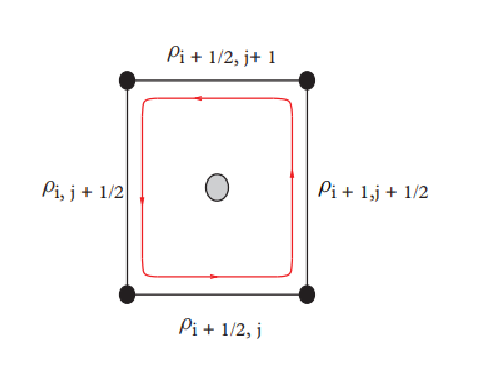
\includegraphics[width=6.5cm,height=4.5cm]{figures/7.eps}
	\caption{}
\end{figure}
取右下角格点坐标为$(i,j)$,用$\rho$来表示图中各处连接,则取闭合回路,有
\begin{equation}
	\rho_{i+\frac{1}{2},j}+\rho_{i+1,j+\frac{1}{2}}-\rho_{i+\frac{1}{2},j+1}-\rho_{i,j+\frac{1}{2}}=0
\end{equation}
这对应了旋度为0的离散版本,同样我们也可以用一个参量来描述它
\begin{equation}
\rho_{i+\frac{1}{2},j}=\phi_{i+1,j}-\phi_{i,j}
\end{equation}
\begin{equation}
	\rho_{i,j+\frac{1}{2}}=\phi_{i,j+1}-\phi_{i,j}
\end{equation}
若我们考虑$(i,j)$出发射的四条线,其自然对应了散度为0的离散版本
\begin{equation}
	\rho_{i+\frac{1}{2},j}-\rho_{i-\frac{1}{2},j}+\rho_{i,j+\frac{1}{2}}-\rho_{i,j-\frac{1}{2}}=0
\end{equation}
同样有
\begin{equation}
	\rho_{i+\frac{1}{2},j}=\psi_{i+\frac{1}{2},j+\frac{1}{2}}-\psi_{i+\frac{1}{2},j-\frac{1}{2}}
\end{equation}
\begin{equation}
	\rho_{i,j+\frac{1}{2}}=-\psi_{i+\frac{1}{2},j+\frac{1}{2}}+\psi_{i+\frac{1}{2},j-\frac{1}{2}}
\end{equation}





%%%%%%%%%%%%%%%%%%%%%%%%%%%%%%%%%%%%%%%%%%%%%%%%%%%%%%%%%%%
%%%%%%%%%%%%%%%%%%%%%%%%%%%%%%%%%%%%%%%%%%%%%%%%%%%%%%%%%%%
%%%%%%%%%%%%%%%%%%%%%%%%%%%%%%%%%%%%%%%%%%%%%%%%%%%%%%%%%%%



\end{document}

%%%%%%%%%%%%%%%%%%%%%%%%%%%%%%%%%%%%%%%%%%%%%%%%%%%%%%%%%%%

